
\documentclass[a4paper]{article} %
\usepackage{graphicx,amssymb} %
\usepackage[latin1]{inputenc}

\textwidth=15cm \hoffset=-1.2cm %
\textheight=25cm \voffset=-2cm %

\pagestyle{empty} %

\date{} %

\def\keywords#1{\begin{center}{\bf Keywords}\\{#1}\end{center}} %

\def\titulo#1{\title{#1}} %
\def\autores#1{\author{#1}} %

% Please, do not change any of the above lines








\usepackage{graphicx}
\graphicspath{%
    {converted_graphics/}% inserted by PCTeX
    {/}% inserted by PCTeX
}
\begin{document}

% Type down your paper title
\titulo{Designing Hamiltonian Cycles}

% Authors
\autores{Francisco de Arriba, Eusebio Corbacho, Ricardo Vidal \\ %
       University of Vigo (Spain) % Affiliation 1
       \\ % If any other author with different Affilation
        \\ \\ % Affiliation 2 (if needed)
       % New author \\
       % New affiliation \\
       % Add authors and affiliation as needed
       \tt{corbacho@uvigo.es}\\
        % Only one corresponding e-mail
       }%


\maketitle

\thispagestyle{empty}



% The abstract

\begin{abstract}Historically, the minimal length Hamiltonian cycles in a random point cloud lying inside a given rectangle are computed by partitioning this rectangle. We have used successive convex hulls of the set of points, in order to obtain partitions better suited for this purpose. The free computer algebra system Sage has been very useful to perform the corresponding computations (for sets of 100 to 200 points, the result is obtained in just 15 seconds using a laptop computer running Ubuntu 12.04 with an Intel Core i7-2630QM processor and 8GB of RAM).\\

The code developed is also applied with success to obtain  good approximations of minimal length Hamiltonian cycles, across the major cities of the countries of the European Union. In each country, $E_i$, we make a transverse Mercator representation centered in the point $C_i$ of average latitude and average longitude among the selected cities in the country. For a list of countries $[E_1,\cdots,E_n]$ we paste in the origin of the complex plane the local chart of $E_1$. Then, the local chart of $E_2$ is translated by the complex number whose modulus is the geodesic distance $(C_1,C_2)$ and whose argument is the angle between the maximal circle $(C_1,C_2)$ and the parallel of $C_1$, and so successively until $E_n$. In this way, all the cities are transformed into a set of points in the complex plane where each pair can be connected by a straight line.
\end{abstract}
\keywords{Hamiltonian Cycle, Convex Hull, Jarvis algorithm modified, Sage, Geographic Coordinates, Geodesic Displacement }
\newpage
\section{Introduction}
The search of minimal length paths which pass just once through each one of the points of a finite subset of the complex plane, $L$, is a classical problem not yet solved in a reasonable computation time, when the cardinal $|L|$  is big.\\
If $R$ is a bounded rectangle containing $L$, good approximations to the optimal solution have been achieved using rectangular partitions $\{R_i \,|\ i\in I\}$ of $R$ which induce partitions $\{L_i\,|\, i\in I\}$ in $L$ so that $L_i=L\cap R_i$ and $|L_i|<k\quad\forall i\in I$ with $k$ a small natural number. In these subsets $L_i$ you can easily find minimal length hamiltonian paths and the standard computations are guided by different strategies to adequately connect the optimal paths for each $L_i$ and generate the desired optimal hamiltonian cycle in all $L$ \cite{H-P}.\\\\
In this communication we present a non-standard attempt of construction of the optimal hamiltonian cycle in any finite set $L$ of the complex plane, based on the following ideas:
\begin{enumerate}\label{COND1}
  \item If $co(L)$ is the convex envelope of $L$, $\partial(co(L))$ is its border and $L\subset \partial(co(L))$ we should just choose an orientation in that border and, according to it, order the points of $L$. In this way we construct a closed hamiltonian path in $L$ which will be of minimal length because it is the only one without crossing of edges.
  \item If there exists a  $z_0\in L$  such that $L'=L\setminus\{z_0\}$ has the property expressed in  \ref{COND1}, we can construct an optimal hamiltonian path in $L'$ and replace the most suitable edge $(z_i,z_{i+1})$ by the polygonal path $(z_i,z_0,z_{i+1})$ so that the new path, which obviously would still be hamiltonian, enlarged its length as little as possible.
  \item \label{COND2} If there existed a $\{z_0,\cdots,z_n\}\subset L$ such that $L'=L\setminus\{z_0,\cdots,z_n\}$ had the property expressed in  \ref{COND1}, we could consider the optimal hamiltonian path in $L'$ and study the order to incorporate the $z_i$ to the path $L'$ to preserve the hamiltonian character and to enlarge its length as little as possible.
  \end{enumerate}
In any $L$ we can find the subset $L_1=L\cap \partial (co(L))$  which obviously has the property expressed in  \ref{COND1}. We add the elements of $L\setminus L_1$ following the heuristic in \ref{COND2}, in order to find the optimal hamiltonian cycle of $L_1$. The elements of $L_2 = L\cap\partial (co(L\setminus L1 ))$ are added in such a way that provide the best Hamiltonian cycle in $L_{12} = L_1\cup L_2$ . We add the elements of $L_3=L\cap \partial (co(L\setminus L_{12}))$ and, so on. A Sage implementation of these ideas can be seen in \cite{A-C-V}.
\\In section 2 we describe some of these algorithms and discuss some examples of use in order to highlight their good computing times in an average laptop. In section 3 we present a simulation of optimal touristic or transport circuits through cities of the European Union so that the results can be compared with those offered in Internet by known sources of geographical information.
\section{Hamiltonian Cycles}
The function {\it listacomplejos(R,n)} returns a random list of $n$ complex numbers contained in the central square of side $2R$ which will be our working set $L$. The function {\it envolturaconvexa(L)} returns the set $L_1=L\cap \partial (co(L))$ counterclockwise ordered and the function {\it cebolla(L)}  returns the list $[L_1 , L_2 , \cdots , L_n ]$ expressing the desired partition of L.\\
The function {\it pegalistas($L_1,L_2$)} returns the set $L_{12}$ as an ordered list which tries to be the best possible hamiltonian cycle in the two first layers. The order of incorporation of the points of $L_2$ to $L_1$ is decided by the minimal length enlargement of the path. Ties are solved by the maximal incorporation angle and, if they persist, we use a recursive algorithm. Once decided the incorporation of a certain $w\in L_2$ between the points $(z_i,z_{i+1})$ of $L_1$ one replaces the piece $[z_{i-1},z_i,w,z_{i+1},z_{i+2}]$ by their optimal reordering and procceds to incorporate a new element of $L_2$.\\
The function cicloham(L) obtains the list $[L_1 , L_2 , \cdots, L_n ]$, computes $L_{12}$ pasting $L_2$ to $L_1$ , $L_{123}$ pasting $L_3$ to $L_{12}$ and, by iteration, proposes as optimal hamiltonian cycle in $L$ the list $L_{1\cdots n}$.\\
Our trust in this technique grew by its good work even in cases whose geometry did not suggest it. For example, if $E$ is the set\\
\newpage
\begin{figure}[h] % float placement: (h)ere, page (t)op, page (b)ottom, other (p)age
  \centering
  % file name: C:/Users/Usuario/Desktop/CORBACHO_ACA2013/fig4.pdf
  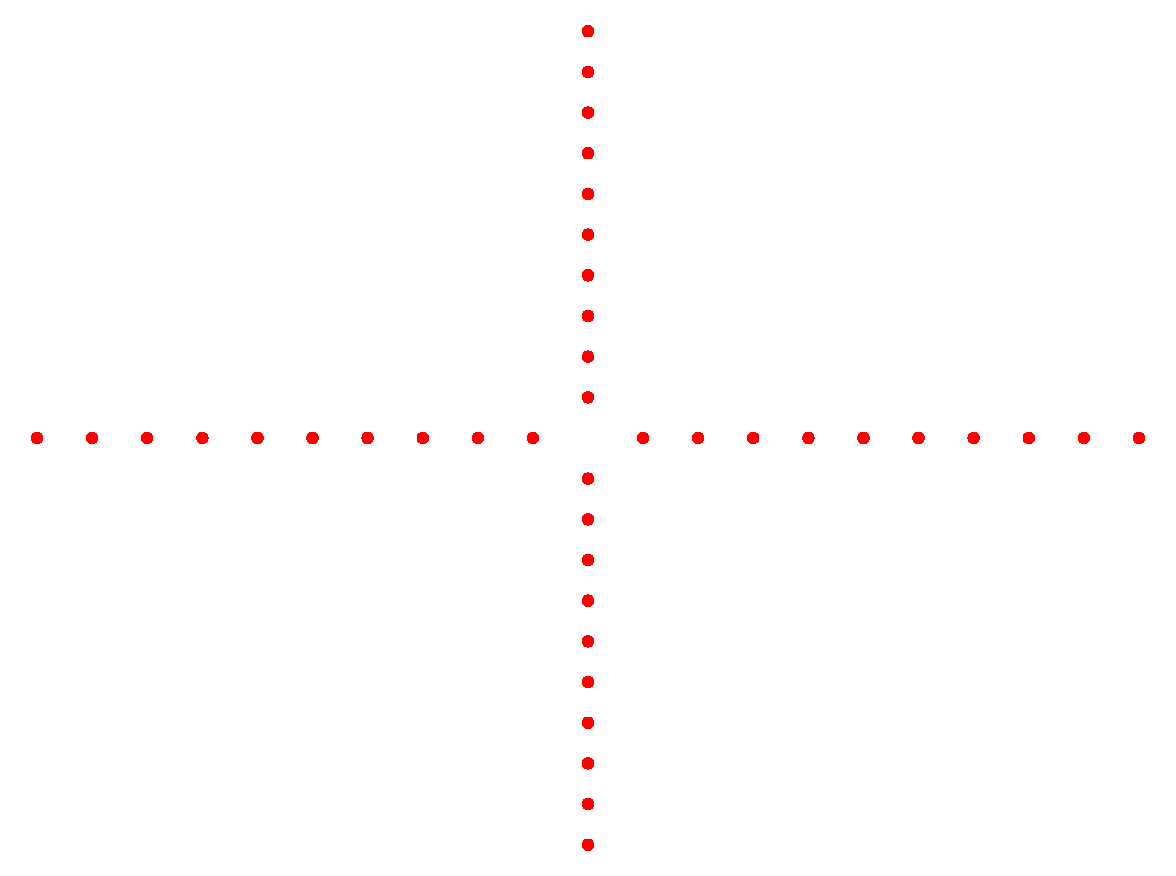
\includegraphics[bb=7 7 558 414,width=2.73in,height=2.01in,keepaspectratio]{fig4}
  \caption{The set E}
\end{figure}
the hamiltonian cycle $Q=cicloham(E)$ is \\
\begin{figure}[h] % float placement: (h)ere, page (t)op, page (b)ottom, other (p)age
  \centering
  % file name: C:/Users/Usuario/Desktop/CORBACHO_ACA2013/fig5.pdf
  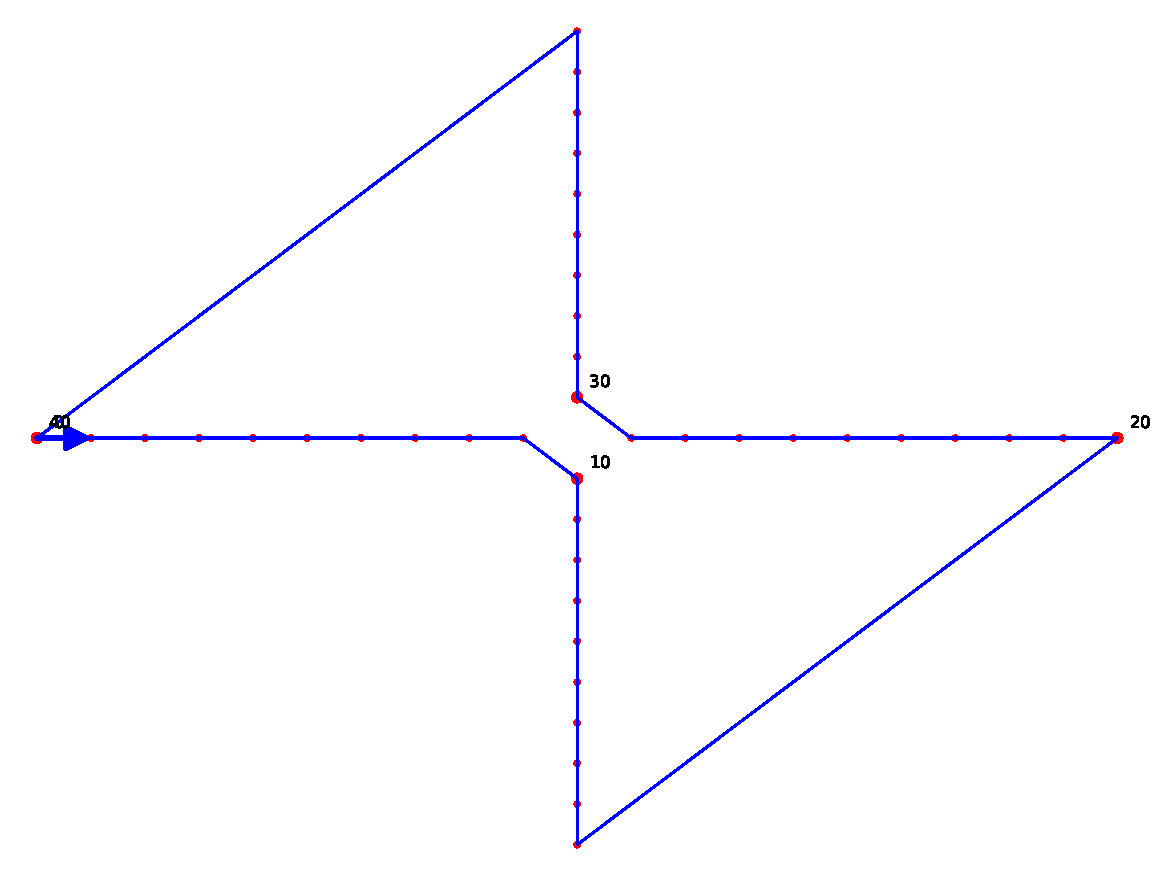
\includegraphics[bb=7 7 558 414,width=2.73in,height=2.01in,keepaspectratio]{fig5}
  \caption{The cicle Q found in set E}
\end{figure}\\\\
which, evidently, is the optimal one.\\
However, in spite of being cautious in the process of pasting, the list $L_{1\cdots n}$ which always is a hamiltonian cycle, can present some crossings of edges and, so, not be the minimal length one. For example, if $L$ is a set with $|L|=400$ in a 40 m length sided square,\\
\begin{figure}[h] % float placement: (h)ere, page (t)op, page (b)ottom, other (p)age
  \centering
  % file name: C:/Users/Usuario/Desktop/CORBACHO_ACA2013/fig1.pdf
  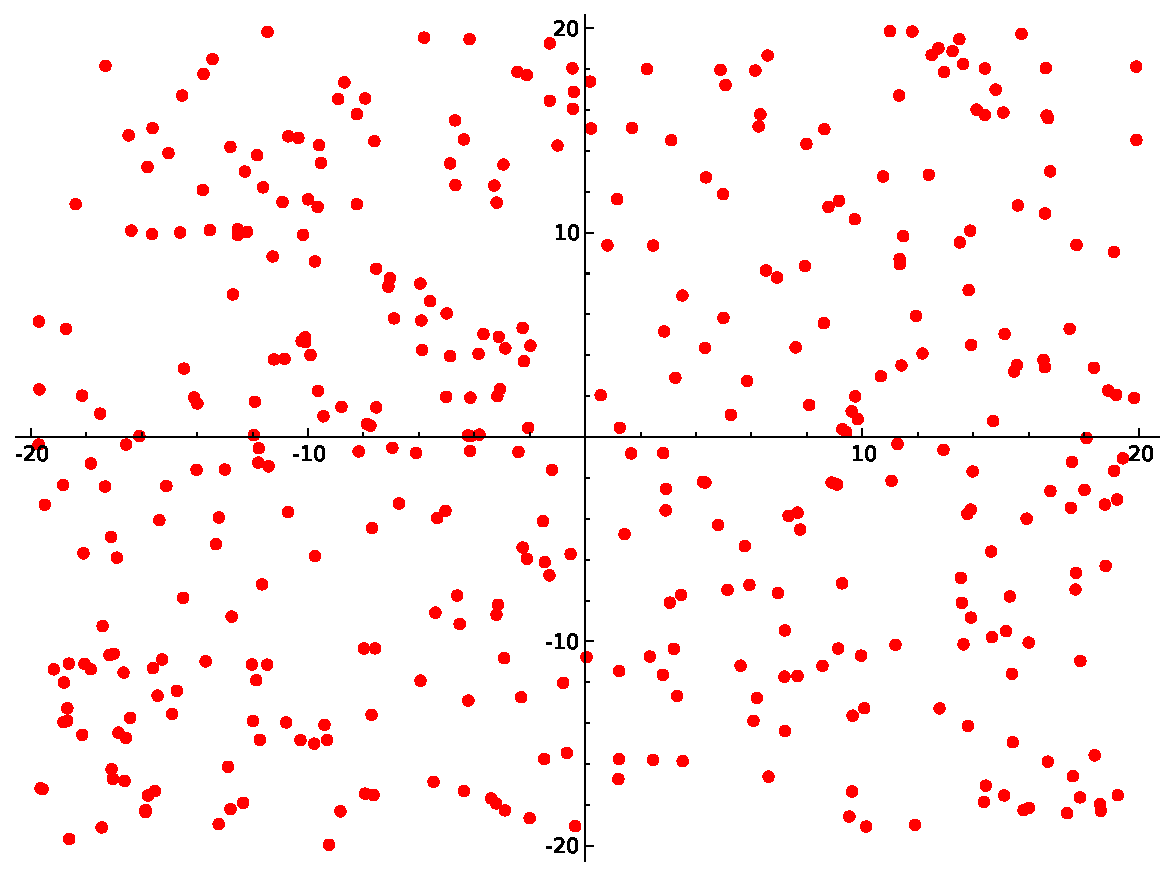
\includegraphics[bb=7 6 557 414,width=2.73in,height=2.03in,keepaspectratio]{fig1}
  \caption{A set L of 400 cities}
\end{figure}\\
\newpage\quad
\noindent
{C=\it cicloham(L)} is a Hamiltonian cycle  with a 654.54 m length which presents two crossings :\\
\begin{figure}[h] % float placement: (h)ere, page (t)op, page (b)ottom, other (p)age
  \centering
  % file name: C:/Users/Usuario/Desktop/CORBACHO_ACA2013/fig2.pdf
  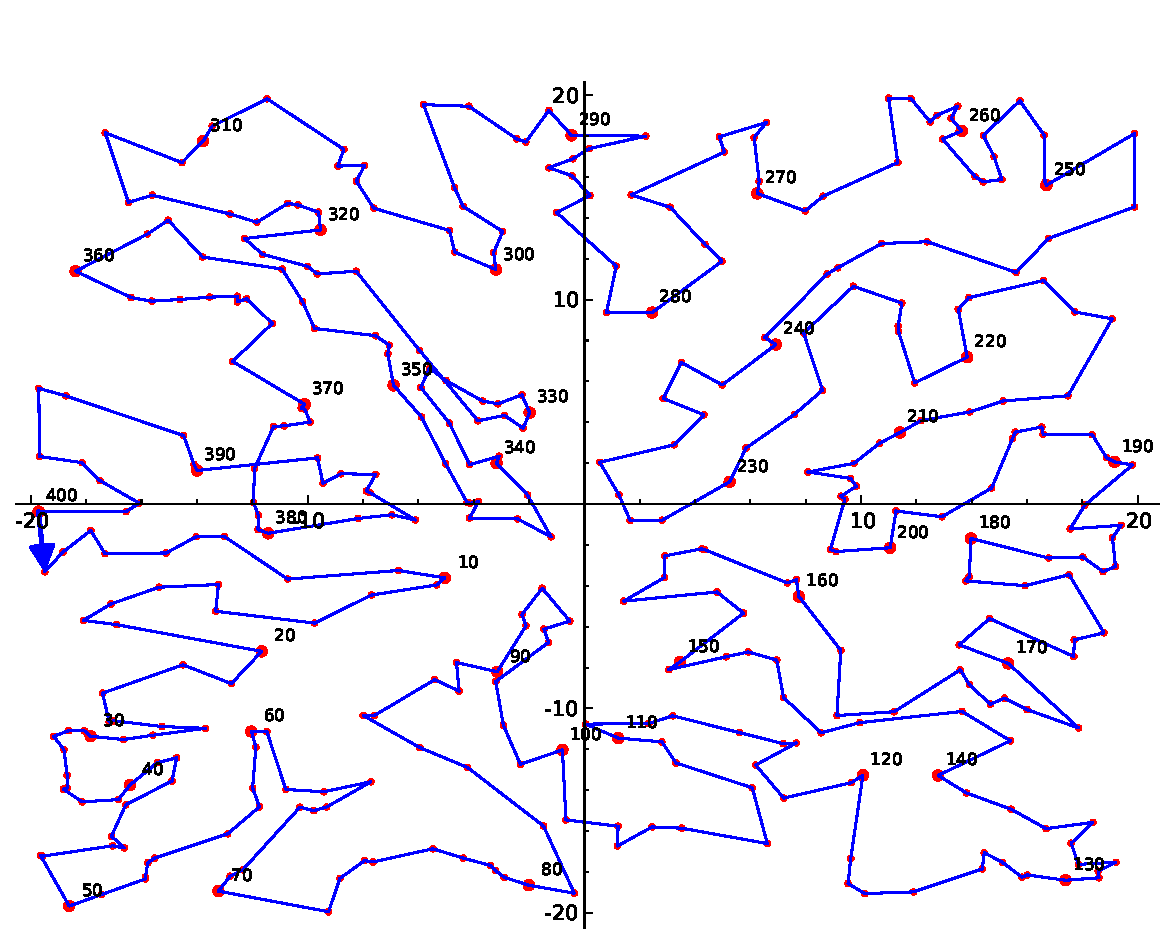
\includegraphics[bb=7 6 557 414,width=2.73in,height=2.02in,keepaspectratio]{fig2}
  \caption{The cycle C found in L}
\end{figure}\\
However we can paste again the piece $C[325:335]$ to the cycle $C[:325]+C[335:]$ by means of the formula {\it MC=mejoratramo(C,325,335)} and the piece $MC[370:390]$ to the cycle $MC[:370]+MC[390:]$ and obtain a cycle  {\it OC=mejoratramo(MC,370,390)} without crossings of 648.92 m.\\
\begin{figure}[h] % float placement: (h)ere, page (t)op, page (b)ottom, other (p)age
  \centering
  % file name: C:/Users/Usuario/Desktop/CORBACHO_ACA2013/fig3.pdf
  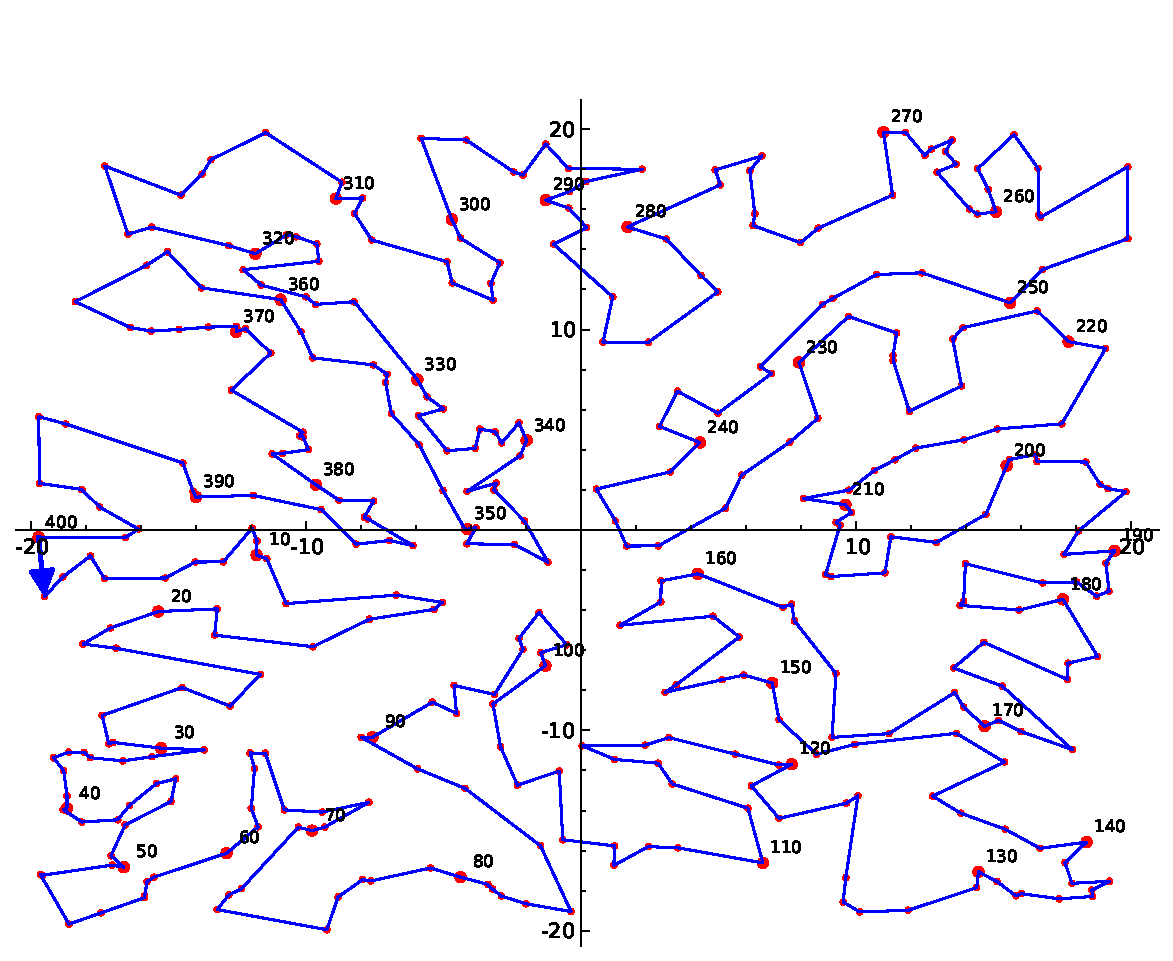
\includegraphics[bb=7 6 557 414,width=2.73in,height=2.02in,keepaspectratio]{fig3}
  \caption{The cycle OC in L without crossings}
\end{figure}\\
Despite this technique does not assure finding the shortest hamiltonian path, its iteration gives a fair approximation if a suitable collaboration man-machine is established. Although the quantification of the goodness of this approximation is currently ongoing work, the heuristics makes us sure that our technique can be used in games of the type \cite{TSP} without the limitation $|L|\leq 50$.
\section{Hamiltonian trips}
One of the more used applications of this type of problems is the design of touristic tours or routes of transport across a certain set of cities. In our case, we have tried to get that the representation of the cities in the complex plane can be realized simply from their latitude and longitude, to make it easy to the user to incorporate cities or places of his interest to the set of the 518 cities of the European Union considered by us.\\
In each country of the EU we have chosen one city per each million of inhabitants, and for that reason we have left Cyprus and Malta out. In the country $E_i$, we make a transverse Mercator representation centered in the point $C_i$ of average latitude and average longitude among the selected cities in the country. For a list of countries $[E_1,\cdots,E_n]$ we paste in the origin of the complex plane the local chart of $E_1$. The local chart of E2 is then translated by the complex number whose modulus is the geodesic distance $(C_1,C_2)$ and whose argument is the angle between the maximal circle $(C_1,C_2)$ and the parallel of $C_1$, and so successively until $E_n$. This is realized by the function {\it viaje($[E_1,\cdots,E_n]$)} which uses, as auxiliary function, the function {\it desplazamiento($E_i,E_{i+1}$)}.\\ The cartographical representation of the cities so obtained is also not standard and we have designed it to make it easy to the user the incorporation of new groups of cities. We think that the small distortions introduced by this representation should not affect the searched optimal hamiltonian cycle although eventually they can modify its real length.\\
For example, the best Hamiltonian cycle across the cities of Spain and Portugal which we obtain with {\it viaje([espanha,portugal])} and a iterated use of the function {\it mejoratramo} is\\
\begin{figure}[h] % float placement: (h)ere, page (t)op, page (b)ottom, other (p)age
  \centering
  % file name: C:/Users/Usuario/Desktop/CORBACHO_ACA2013/fig6.pdf
  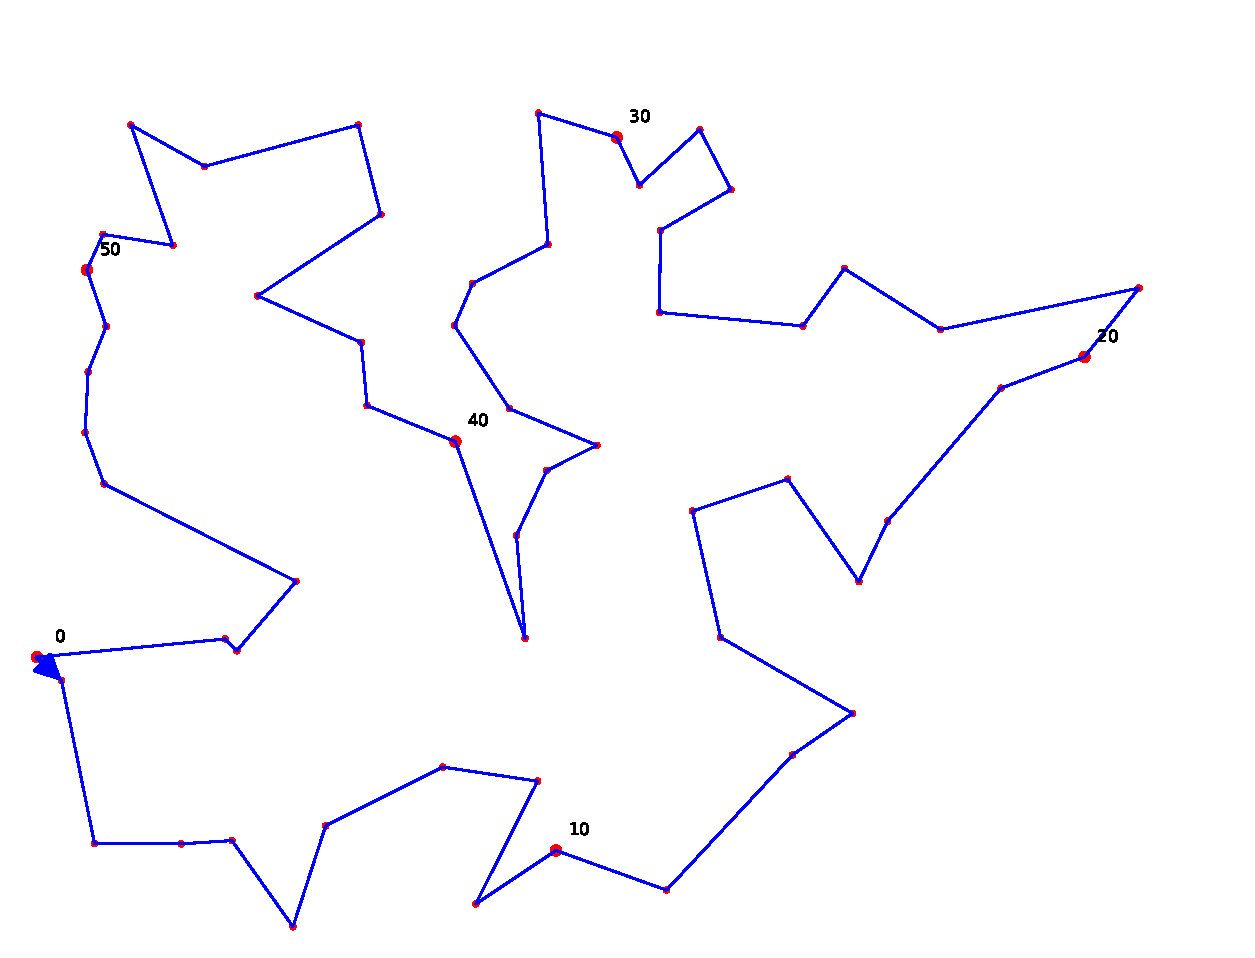
\includegraphics[bb=7 7 558 414,width=2.73in,height=2.01in,keepaspectratio]{fig6}
  \caption{The cicle Spain and Portugal}
  \end{figure}\\
{\small $0\quad \,\,\,[ LISBOA, Setubal, Portimao, Tavira, Huelva, Cadiz, Sevilla, Cordoba, Jaen,  Malaga]$\\
$10\quad [ Granada, Almeria, Murcia, Alicante, Albacete, Cuenca, Teruel, Valencia, Castellon, Tarragona ]$\\
$20\quad [ Barcelona, Gerona, Lerida, Huesca, Zaragoza, Soria, Logronho, Pamplona, S.Sebastian, Vitoria ]$\\
$30\quad [ Bilbao, Santander, Burgos, Palencia, Valladolid, Segovia, Guadalajara, MADRID, Toledo, Ciudad\, \,Real ]$\\
$40\quad [ Avila, Salamanca, Zamora, Bragansa, Leon, Oviedo, Lugo, Corunha, Orense, Pontevedra ]$\\
$50\quad [Valensa, Braga, Porto, Aveiro, Coimbra, Caceres, Badajoz, Elvas, LISBOA ]$}\\\\
with a 5502.95 km length and the cities sequenced by groups of ten, to easily localize them in the graphic. Undoubtedly it seems to us more trustful the sequencing of the cycle than its length. This would be a minor question because in our planning we have taken into account neither the orography nor the road net. However, the number of cities seems to be enough to suppose that for each edge of the cycle there exists a road of the net which connects the two cities at its endpoints.
\begin{thebibliography}{00}
\bibitem {H-P} Har-Peled, S. ; \textit{ Geometric Approximation Algorithms}, AMS Mathematical Surveys and Monographs Vol 173,  (2011).
\bibitem {A-C-V} Arriba, F. Corbacho, E. Vidal, R. \textit{https://dl.dropboxusercontent.com/u/21326323/ACA2013.sws}
\bibitem {TSP} TSP Games \textit{(http://www.tsp.gatech.edu/games/index.html}
\end{thebibliography}


\end{document}
